\chapter{Preliminaries}
\label{cha:prelims}

\section{Drug Management}
\label{sec:drug-management}

To get a better understanding what the term Drug Management stands for it is essential to clearify the term Management at first.
In general management comprises the non-executing tasks of a certain domain to accomplish certain goals.
These non-executing tasks are divided in the four stages: \textit{planning}, \textit{organizing}, \textit{leading} and \textit{controlling} \cite{robbins2007fundamentals}.
The term Drug Management was adopted by the WHO in their publication about managing drugs at health centres \cite{who2004}.
The term management is defined in their publication as follows: 
\begin{quote}
  Management is the act or art of being responsible or in charge and conducting or supervising something (e.g. a health centre pharmacy, business, public undertaking) with a degree of skill and address. It is the judicious use of means to accomplish an end (i.e. public health).
\end{quote}
With this definition in mind the question can be answered why it is useful to manage drugs.
Refering to the WHO there are three main reasons:
\begin{enumerate}
\item ``Firstly, drugs are part of the link between the patient and health services.''\\
  This is the most trivial reason that addresses the direct influence of drugs to the patients health state. If drugs are not managed properly the success of the treatment process is imperiled. 
\item ``Secondly, poor drug management [...] is a critical issue, but major improvements are possible that can save money and improve access.''\\
  Besides the medical benefits, a proper drug management can also result in financial advantages. These can be achived by an improved selection and procurement of the required drugs.
\item ``Finally, drugs are no longer the responsibility of health workers only.''\\
  This fact is based on a progress in the last couple of years that led to a broader self-determination of patients. 
  Therefore the claim to be involved in the drug selection process and to have an overview of the currently prescribed drugs requires an adequate drug management of all involved players.
\end{enumerate}
\begin{figure}
  \centering
  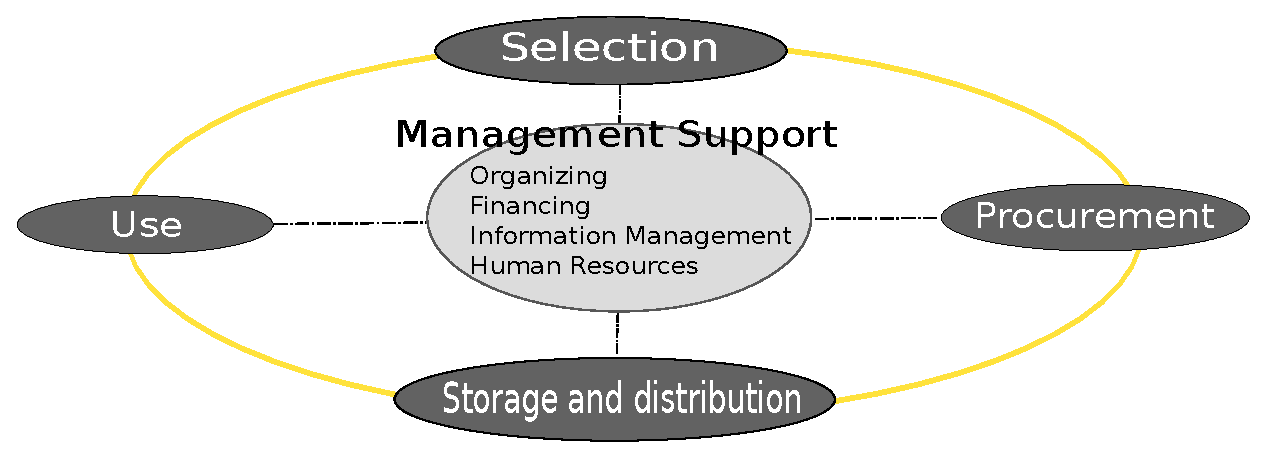
\includegraphics[width=\textwidth]{preliminaries/life_cycle.eps}
  \caption{WHO drug management life cycle}
  \label{fig:life_cycle}
\end{figure}
The WHO proposes a drug management life cycle which is the foundation to implement a proper drug management at a certain institution.
This life cycle which is shown in figure \ref{fig:life_cycle} contains four phases which are described shortly in the following listing:
\begin{itemize}
\item Selection\\
  Selection comprises the process of choosing the right drug regarding the patient's symptoms and other circumstances like already prescribed drugs or drug allergies.
  If all possible circumstances are considered properly, this phase can be the most comprehensive of the cycle.
\item Procurement\\
  After the right drugs where chosen in the selection phase the next step is to procure these drugs.
  In this phase drug management can help to chose the best, e.g. cheapest vendors.
  Otherwise it may be the case that more expensive vendors are chosen just because of the large sector of drug companies.
\item Use\\
  Many adverse drug events occur because of incorrect delivered drugs.
  Examples are too high dosages or incorrect routes of administration.
  The goal of the third phase therefore is to provide the right information about the usage of a drug at the right place to the right time.
\item Storage and distribution\\
  The fourth phase manages how drugs are stored.
  This is important to prevent disfigurations of labels and to ``maintain integrity of packaging and so guarantee quality and potency of drugs during shelf life''.
  Further the patient needs help in cases of losing the drug packaging or similar cases.
\end{itemize}
According to the WHO these phases ``are interlinked and are reinforced by appropriate management support systems (i.e. tools)''.
The API which is developed by this thesis is settled up in this category of support systems.

One point has to be remarked regarding the scope of the WHO recommendations.
Althought the cited publication addresses health centres, recommendations like the life cycle are easily adoptable to other areas, e.g. private healthcare.

\section{Semantic Web}
\label{sec:semantic-web}
The ongoing growth of digital data in the past years has revealed many shortcomings that occur with these amounts of data.
Fields of research like \textit{Big Data} also show the importance of managing these amounts of data efficiently.
One key issue since years is the distinction between syntactically and semantically processable data.
Tim Berners-Lee proposed in 2001 a concept to describe specific data statements in a better way \cite{berners2001semantic}.
This model behind this approach was called \textit{Ressource Description Framework} (RDF) \cite{klyne2004resource} and is one important part of the Semantic Web Stack.
This stack combines several technologies and standars that are necessary to transfer the syntactic web to a semantic web.
The Semantic Web Stack is illustrated in figure \ref{fig:sem_stack}.
\begin{figure}
  \centering
  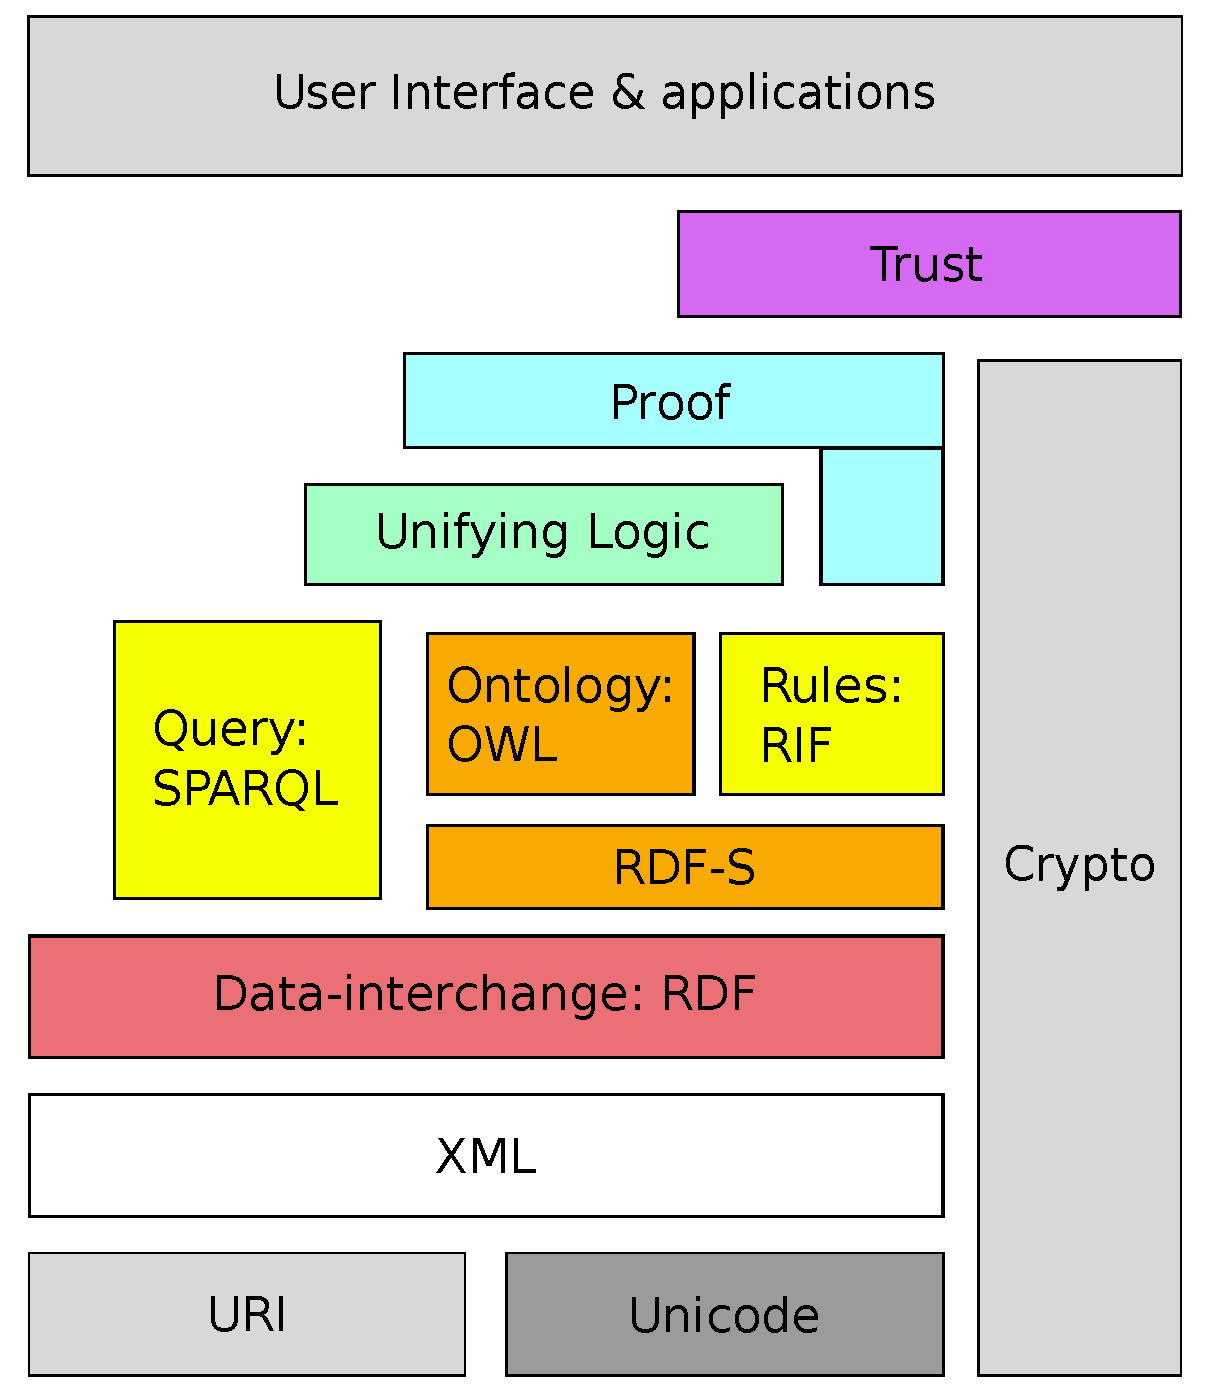
\includegraphics[scale=0.3]{preliminaries/semweb_stack}
  \caption{Semantic Web Stack}
  \label{fig:sem_stack}
\end{figure}
The advantages of a semantic web are numerous.
The main advantage is that the information are not only machine readable but machine processable.
This entails other improvements like reasoning that transfers implicit knowledge into explicit.

The following paragraphs will describe the most important technologies and standards of the Semantic Web Stack that are necessary for this thesis:

At the lowest level of the stack there is the concept of the Uniform Resource Identifier (URI).
A URI identifies a specific resource, e.g. a car.
For several other domains there already exists such concepts as URIs.
For example the Uniform Resource Locator (URL) identifies web sites or an International Standard Book Number (ISBN) identifies books.
The URI itself is just a set of characters that can be additionally divided into five segments: scheme, authority, path, query and fragment.
An example of such a URI would be: \texttt{http://example.com/Alice}.
This URI would describe the resource ``Alice''.

Based on the identification of resources, the already mentioned Resource Description Framework has the goal to describe these resources.
Therefore RDF is one of the most important concepts of the Semantic Web Stack.
The approach of RDF to model knowledge is to express statements as triples.
This is tight to how natural language is mostly constructed.
Obviously that is why the components of the triple use the well known names of \textit{Subject, Predicate} and \textit{Object}.
Figure \ref{fig:sem_rdf} shows an example triple.
The subject of such a triple has to be always an URI, same belongs to the predicate.
An exception is the object which can be additionally a literal.
A literal is a direct information typed in a specific way, e.g. as date or simply text, which refers to no other resource.
For more advanced models it is possible to describe the subject and object in a anonymous way, without a concrete entity.
These anonymous resources are called blank nodes, but will be without broader relevance for this thesis.
At the end one important distinction has to be made about RDF.
Often RDF is getting confused with RDF/XML \cite{beckett2004rdf} -- a notation of RDF statements.
While RDF itself only describes how to model information, several RDF notations exist that express these information in several ways.
Examples for such notations besides the already mentioned RDF/XML is N-Triples, Turtle \cite{beckett2008turtle} or JSON-LD \cite{lanthaler2012using}.

\begin{figure}
  \centering
  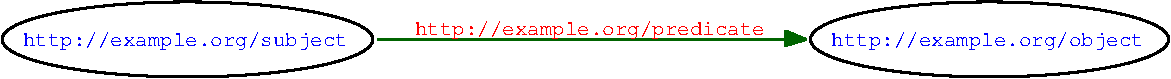
\includegraphics[width=\textwidth]{preliminaries/semweb_rdf1}
  \caption{Example of a RDF triple}
  \label{fig:sem_rdf}
\end{figure}

On top of RDF the Semantic Web Stack levels SPARQL, an RDF query language.
SPARQL enables comprehensive queries over a knowledge base built on RDF.
SPARQL itself uses many well known keywords from SQL, but because of the graph structure of RDF and therefore of the triple stores the languages naturally differ.\\
Given the following two triples in Turtle notation:
\begin{lstlisting}[numbers=none,caption=Example Turtle triples]
@prefix ex: <http://example.com/>.
ex:anna ex:name ``Anna''.
ex:bob  ex:name ``Bob''. 
\end{lstlisting}
Then the following simple SPARQL query would return the result ``Bob''.
\begin{lstlisting}[numbers=none,caption=Example SPARQL query]
SELECT ?name
WHERE {
  ex:bob ex:name ?name.
}
\end{lstlisting}

With SPARQL 1.1 so called \textit{Federated Queries} were introduced.
These Federated Queries are Statements that are queried against multiple (federated) SPARQL endpoints.
This is a key feature for an easy integration of several RDF graphs.

\section{Linked Open Data}
\label{sec:linked-open-data}
As described in the previous section RDF statements spans a graph of triples.
Thereby, each knowledge base spans their own graph.
Examples for large knowledge bases are DBpedia\footnote{\url{http://dbpedia.org} (last access Sept 18, 2013)}, LinkedGeoData\footnote{\url{http://linkedgeodata.org} (last access Sept 18, 2013)} or Drugbank.
\textit{Linked Data} in general now describes the situation that entities of one knowledge base link to entities of another knowledge base.
For example an entity of DBpedia about a drug could link to the same entity in Drugbank for further information.
In this case both knowledge bases would describe the same entity.
In other cases Linked Data is used to refer to different entities.
In the example above this could mean that the drug entity of Drugbank is refering to an entity of a chemical knowledge base to describe the compund of the drug in more detail.
Listing \ref{linkedturtle} shows an example given in Turtle notation where an RDF triple links from one knowledge base to another.
This triple states that the DBpedia entity ``Metoprolol'' describes the same subject as the Drugbank entity ``Metoprolol''.
\begin{lstlisting}[numbers=none,caption=Example triple for linking two entities of different knowledge bases,label=linkedturtle]
@prefix drugbank: <http://drugbank.bio2rdf.org/>
@prefix dbpedia: <http://dbpedia.org/resource/>
@prefix owl: <http://www.w3.org/2002/07/owl#>

dbpedia:Metoprolol owl:sameAs drugbank:Metoprolol.
\end{lstlisting}
If the mentioned knowledge bases are freely available and usable then this is called \textit{Linked Open Data} (LOD).

Tim Berners-Lee proposed some rules\footnote{\url{http://www.w3.org/DesignIssues/LinkedData.html} (last access Sept 18, 2013)} that state whether a data source is Linked Open Data, or not.
These rules are:
\begin{enumerate}
\item Use URIs to denote things.
\item Use HTTP URIs so that these things can be referred to and looked up ("dereferenced") by people and user agents.
\item Provide useful information about the thing when its URI is dereferenced, leveraging standards such as RDF, SPARQL.
\item Include links to other related things (using their URIs) when publishing data on the Web.
\end{enumerate}

Further, Berners-Lee categorizes Linked Open Data on the basis of a five star rating.
Therefore the more a knowledge base follows these principals the more stars it earns.
\begin{itemize}
\item \textbf{1 star} - Available on the web (whatever format) but with an open licence, to be Open Data
\item \textbf{2 stars} - Available as machine-readable structured data (e.g. excel instead of image scan of a table)
\item \textbf{3 stars} - as (2) plus non-proprietary format (e.g. CSV instead of excel)
\item \textbf{4 stars} - All the above plus, Use open standards from W3C (RDF and SPARQL) to identify things, so that people can point at your stuff
\item \textbf{5 stars} - All the above, plus: Link your data to other people’s data to provide context
\end{itemize}

\begin{figure}
  \centering
  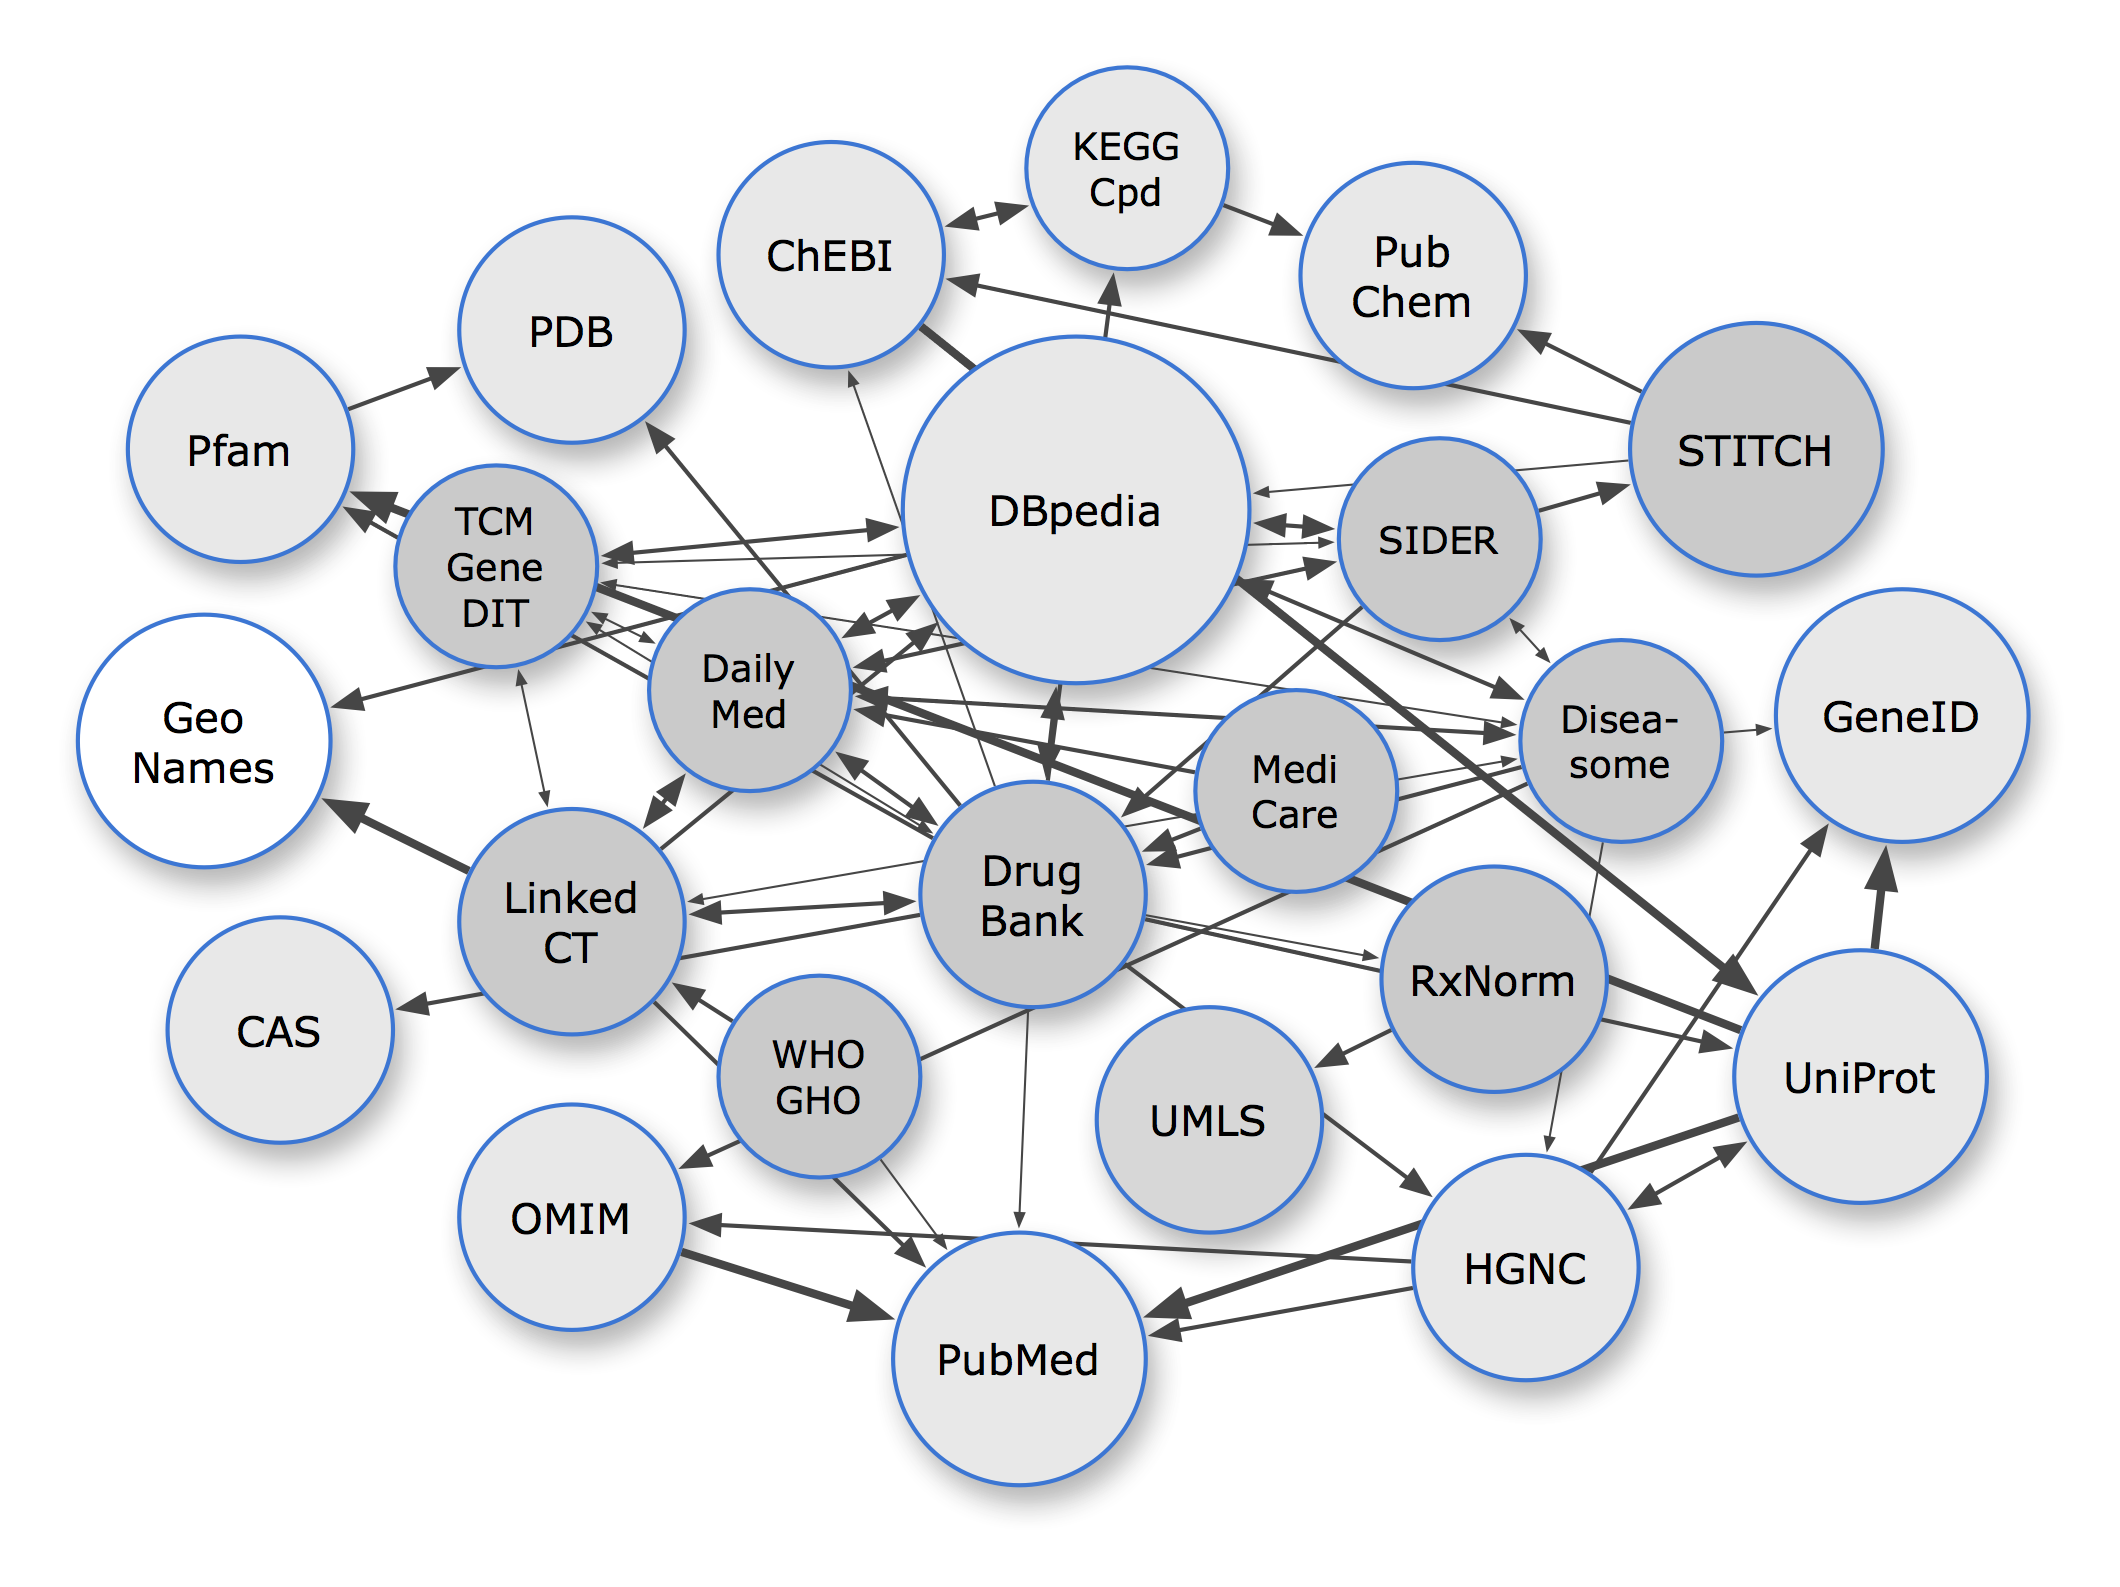
\includegraphics[scale=0.7]{preliminaries/2010-12-04_lodd_cloud.png}%lod-cloud}
  \caption{Biomedical data sets of the Linked Open Data cloud}% diagram, by Richard Cyganiak and Anja Jentzsch. http://lod-cloud.net/}
  \label{fig:lod_cloud}
\end{figure}


In conjunction with SPARQL this leads to large federated collections of knowledge that are comprehensively queryable.
Figure \ref{fig:lod_cloud} gives an overview over the biomedical domain of the Linked Open Data cloud in 2010.
But this is only a small section of the complete Linked Open Data cloud and produces such graphs for the complete cloud is going to be unreadable in the last years.
%But this kind of figure will end soon because of the rapidly evolving number of data sets.

%%% Local Variables: 
%%% mode: latex
%%% TeX-master: "../thesis"
%%% End: 
